\documentclass[a4paper,12pt]{article}
\usepackage[utf8]{inputenc}
\usepackage[english]{babel}
\usepackage{amsmath,amssymb}
\usepackage{geometry}\geometry{margin=2.5cm}
\usepackage{enumitem}
\usepackage{booktabs}
\usepackage{tikz}
\usetikzlibrary{arrows.meta, positioning, calc, decorations.pathreplacing}
\usepackage{pgfplots}\pgfplotsset{compat=1.18}
\usepackage{tcolorbox}
\tcbuselibrary{breakable}
\usepackage{xcolor}
\newtcolorbox{begriffe}[1][]{colback=yellow!10, colframe=yellow!60!black, fonttitle=\bfseries, title={What do the terms mean?}, breakable, #1}
\newtcolorbox{wastun}[1][]{colback=orange!5, colframe=orange!60!black, fonttitle=\bfseries, title={What needs to be done?}, breakable, #1}
\newcommand{\piv}[1]{{\color{red}\boxed{#1}}}
\newcommand{\grafik}{\textcolor{gray}{\small\textit{[Graphical explanation -- not part of the solution]}}}
\newcommand{\erglerk}{\textcolor{gray}{\small\textit{[Explanation added]}}}
\newcommand{\EW}{eigenvalue}
\newcommand{\EV}{eigenvector}

\title{Exercise Sheet 12 -- Solutions \\ \large Linear Algebra}
\author{}
\date{}

\begin{document}
\maketitle

\begin{begriffe}
\begin{itemize}[leftmargin=*, nosep]
    \item \textbf{Diagonalizable}: $A$ is called diagonalizable if there is an \emph{invertible} matrix $P$ and a \emph{diagonal} matrix $D$ with
    \[
    D = P^{-1} A P \qquad\Longleftrightarrow\qquad A = P D P^{-1}.
    \]
    \item \textbf{What are $P$ and $D$?} The \textbf{columns of $P$} are the eigenvectors of $A$. The \textbf{diagonal of $D$} holds the corresponding eigenvalues -- in the \emph{same order} as the columns.
    \item \textbf{Criterion}: An $n\times n$ matrix is diagonalizable $\Leftrightarrow$ there are $n$ linearly independent eigenvectors $\Leftrightarrow$ for \emph{every} eigenvalue $\text{GM} = \text{AM}$ (the eigenspace dimensions sum to $n$).
    \item \textbf{Reminder}: AM $=$ multiplicity as a root of the char.\ polynomial; GM $= \dim$ eigenspace $=$ number of independent eigenvectors for that eigenvalue.
\end{itemize}
\end{begriffe}

\grafik

\begin{center}
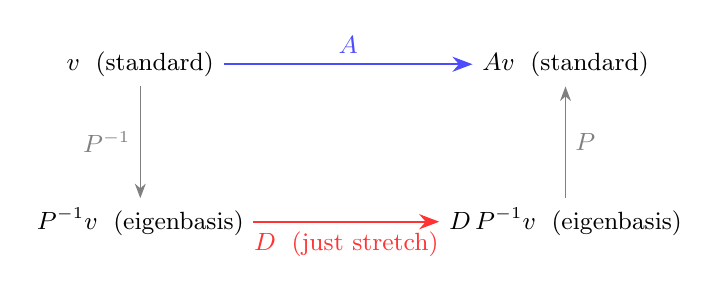
\begin{tikzpicture}[scale=1.0, >={Stealth[scale=1.1]}, every node/.style={font=\small}]
\node (vE)  at (0,2)   {$v$ \;(standard)};
\node (wE)  at (5.4,2) {$Av$ \;(standard)};
\node (vB)  at (0,0)   {$P^{-1}v$ \;(eigenbasis)};
\node (wB)  at (5.4,0) {$D\,P^{-1}v$ \;(eigenbasis)};
\draw[->, blue!70, thick] (vE) -- (wE) node[midway, above]{$A$};
\draw[->, red!80, thick] (vB) -- (wB) node[midway, below]{$D$ \;(just stretch)};
\draw[->, gray] (vE) -- (vB) node[midway, left]{$P^{-1}$};
\draw[->, gray] (wB) -- (wE) node[midway, right]{$P$};
\end{tikzpicture}
\end{center}

\textcolor{gray}{\small\textit{Diagonalizing means: look at $A$ through the right glasses. Instead of applying $A$ directly, go with $P^{-1}$ into the eigenvector basis, where the map is just a \emph{stretch} per axis (the diagonal matrix $D$), then go back with $P$. That is exactly $A = P D P^{-1}$.}}

\bigskip
\hrule
\bigskip

%% ============================================================
\subsection*{Exercise 47}
%% ============================================================

\textbf{Problem.} Are the matrices diagonalizable over $\mathbb{R}$? If yes, give $P$ (invertible) and $D$ (diagonal) with $D = P^{-1}AP$; if no, explain why.
\[
\text{(a)}\ \begin{pmatrix} 4 & 1 & 1 \\ 2 & 5 & 2 \\ -1 & -1 & 2 \end{pmatrix}, \qquad
\text{(b)}\ \begin{pmatrix} 5 & 2 & 3 \\ 2 & 4 & 2 \\ -3 & -2 & -1 \end{pmatrix}, \qquad
\text{(c)}\ \begin{pmatrix} 1 & 0 & 5 \\ 0 & 6 & 0 \\ 1 & 0 & 5 \end{pmatrix}.
\]

\begin{wastun}
\begin{itemize}[leftmargin=*, nosep]
    \item These are exactly the matrices from \textbf{sheet 11} (Exercises 43 and 44). Eigenvalues, AM, GM and eigenspace bases were already computed there -- we start with the \textbf{summary} (table below).
    \item Per matrix only check: \textbf{is GM $=$ AM everywhere?} If yes $\to$ diagonalizable, then $P =$ eigenvectors as columns, $D =$ eigenvalues on the diagonal. If no $\to$ not diagonalizable (too few eigenvectors).
\end{itemize}
\end{wastun}

\textbf{Summary from sheet 11.}
\begin{center}
\begin{tabular}{@{}clll@{}}
\toprule
Matrix & \EW{} $\lambda$ & AM, GM & Basis of the eigenspace \\
\midrule
(a) & $3$ & $2,\,2$ & $(-1,1,0),\ (-1,0,1)$ \\
    & $5$ & $1,\,1$ & $(-1,-2,1)$ \\[2pt]
(b) & $2$ & $2,\,\mathbf{1}$ & $(-1,0,1)$ \\
    & $4$ & $1,\,1$ & $(-1,-1,1)$ \\[2pt]
(c) & $0$ & $1,\,1$ & $(-5,0,1)$ \\
    & $6$ & $2,\,2$ & $(0,1,0),\ (1,0,1)$ \\
\bottomrule
\end{tabular}
\end{center}

\grafik

\begin{center}
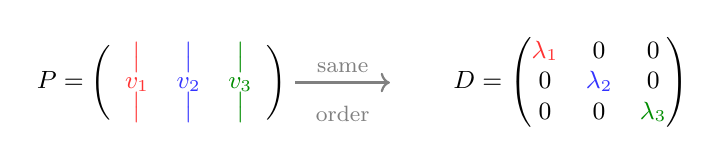
\begin{tikzpicture}[scale=1.0, every node/.style={font=\small}]
\node at (0,0) {$P = \left(\begin{array}{ccc} \color{red!80}\big| & \color{blue!80}\big| & \color{green!55!black}\big| \\[-2pt] \color{red!80}v_1 & \color{blue!80}v_2 & \color{green!55!black}v_3 \\[-2pt] \color{red!80}\big| & \color{blue!80}\big| & \color{green!55!black}\big| \end{array}\right)$};
\node at (5.2,0) {$D = \begin{pmatrix} \color{red!80}\lambda_1 & 0 & 0 \\ 0 & \color{blue!80}\lambda_2 & 0 \\ 0 & 0 & \color{green!55!black}\lambda_3 \end{pmatrix}$};
\draw[->, gray, thick] (1.7,0) -- (2.9,0) node[midway, above]{\footnotesize same};
\node[gray] at (2.3,-0.4){\footnotesize order};
\end{tikzpicture}
\end{center}

\textcolor{gray}{\small\textit{Construction: each column of $P$ is an \EV{}, and at the same spot on the diagonal of $D$ sits its \EW{}. Column $1$ belongs to $\lambda_1$, column $2$ to $\lambda_2$, etc.\ -- the order must match.}}

%% --- 47 (a) ---
\subsubsection*{(a) Matrix $A = \left(\begin{smallmatrix} 4 & 1 & 1 \\ 2 & 5 & 2 \\ -1 & -1 & 2 \end{smallmatrix}\right)$}

\textbf{Diagonalizable?} Eigenvalues $3$ (AM $2$, GM $2$) and $5$ (AM $1$, GM $1$). For both GM $=$ AM, and $2 + 1 = 3$ independent eigenvectors $\Rightarrow$ \textbf{yes, diagonalizable}.

\textbf{Build $P$ and $D$.} I take the three eigenvectors as columns (first the two for $\lambda = 3$, then the one for $\lambda = 5$) and write the eigenvalues in the same order onto the diagonal:
\[
P = \begin{pmatrix} -1 & -1 & -1 \\ 1 & 0 & -2 \\ 0 & 1 & 1 \end{pmatrix}, \qquad
D = \begin{pmatrix} 3 & 0 & 0 \\ 0 & 3 & 0 \\ 0 & 0 & 5 \end{pmatrix}.
\]
\erglerk\ \textcolor{gray}{\small Column 1 $=(-1,1,0)$ and column 2 $=(-1,0,1)$ are the \EV{}s for $3$, column 3 $=(-1,-2,1)$ the one for $5$ -- that is why the diagonal reads $3, 3, 5$.}

\textbf{Check} (instead of computing $P^{-1}$): $D = P^{-1}AP$ is equivalent to $AP = PD$ (just multiply by $P$ from the left). And $AP = PD$ means, column by column: $A v_i = \lambda_i v_i$. That is exactly our eigenvectors:
\[
A\begin{pmatrix}-1\\1\\0\end{pmatrix} = 3\begin{pmatrix}-1\\1\\0\end{pmatrix},\quad
A\begin{pmatrix}-1\\0\\1\end{pmatrix} = 3\begin{pmatrix}-1\\0\\1\end{pmatrix},\quad
A\begin{pmatrix}-1\\-2\\1\end{pmatrix} = 5\begin{pmatrix}-1\\-2\\1\end{pmatrix}. \ \checkmark
\]
\[
\fbox{\parbox{0.93\textwidth}{\centering
$A$ is diagonalizable with
$P = \left(\begin{smallmatrix} -1 & -1 & -1 \\ 1 & 0 & -2 \\ 0 & 1 & 1 \end{smallmatrix}\right)$,
$\ D = \left(\begin{smallmatrix} 3 & 0 & 0 \\ 0 & 3 & 0 \\ 0 & 0 & 5 \end{smallmatrix}\right)$,
\ and $D = P^{-1}AP$.
}}
\]

%% --- 47 (b) ---
\subsubsection*{(b) Matrix $A = \left(\begin{smallmatrix} 5 & 2 & 3 \\ 2 & 4 & 2 \\ -3 & -2 & -1 \end{smallmatrix}\right)$}

\textbf{Diagonalizable?} Eigenvalues $2$ (AM $\mathbf{2}$, GM $\mathbf{1}$) and $4$ (AM $1$, GM $1$). For eigenvalue $2$ we have GM $= 1 <$ AM $= 2$.

\grafik

\begin{center}
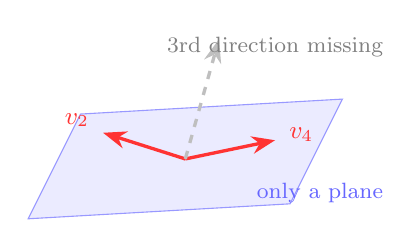
\begin{tikzpicture}[scale=0.95, >={Stealth[scale=1.0]}, every node/.style={font=\small}]
% a plane (span of two eigenvectors) inside R^3, third direction missing
\draw[fill=blue!8, draw=blue!40] (-1.6,-0.7) -- (1.9,-0.5) -- (2.6,0.9) -- (-0.9,0.7) -- cycle;
\draw[->, red!80, very thick] (0.5,0.1) -- (-0.6,0.45);
\draw[->, red!80, very thick] (0.5,0.1) -- (1.7,0.35);
\node[red!80] at (-0.95,0.62){$v_2$};
\node[red!80] at (2.05,0.42){$v_4$};
\node[blue!60] at (2.3,-0.35){\footnotesize only a plane};
% missing third direction
\draw[->, gray!50, very thick, dashed] (0.5,0.1) -- (0.95,1.7);
\node[gray] at (1.7,1.6){\footnotesize 3rd direction missing};
\end{tikzpicture}
\end{center}

\textcolor{gray}{\small\textit{We only have $1 + 1 = 2$ independent eigenvectors (one for $2$, one for $4$). Two directions span only a \emph{plane} in $\mathbb{R}^3$ -- a third direction for a whole basis is missing. So one cannot build a $P$ from eigenvectors.}}

\textbf{Reason.} $A$ would be diagonalizable only with $3$ independent eigenvectors. But we have only $\text{GM}(2) + \text{GM}(4) = 1 + 1 = 2 < 3$. At eigenvalue $2$ an \EV{} ``is missing'' (GM $1 <$ AM $2$).
\[
\fbox{\parbox{0.93\textwidth}{\centering
$A$ is \emph{not} diagonalizable, because $\text{GM}(2) = 1 < \text{AM}(2) = 2$ \\
(only $2$ instead of $3$ independent eigenvectors).
}}
\]

%% --- 47 (c) ---
\subsubsection*{(c) Matrix $A = \left(\begin{smallmatrix} 1 & 0 & 5 \\ 0 & 6 & 0 \\ 1 & 0 & 5 \end{smallmatrix}\right)$}

\textbf{Diagonalizable?} Eigenvalues $0$ (AM $1$, GM $1$) and $6$ (AM $2$, GM $2$). Both GM $=$ AM, $1 + 2 = 3$ independent eigenvectors $\Rightarrow$ \textbf{yes}.

\textbf{Build $P$ and $D$.} Columns: the \EV{} for $0$, then the two for $6$:
\[
P = \begin{pmatrix} -5 & 0 & 1 \\ 0 & 1 & 0 \\ 1 & 0 & 1 \end{pmatrix}, \qquad
D = \begin{pmatrix} 0 & 0 & 0 \\ 0 & 6 & 0 \\ 0 & 0 & 6 \end{pmatrix}.
\]

\textbf{Check} $AP = PD$, column by column ($A v_i = \lambda_i v_i$):
\[
A\begin{pmatrix}-5\\0\\1\end{pmatrix} = \begin{pmatrix}0\\0\\0\end{pmatrix} = 0\cdot v_1,\quad
A\begin{pmatrix}0\\1\\0\end{pmatrix} = 6\begin{pmatrix}0\\1\\0\end{pmatrix},\quad
A\begin{pmatrix}1\\0\\1\end{pmatrix} = 6\begin{pmatrix}1\\0\\1\end{pmatrix}. \ \checkmark
\]
\[
\fbox{\parbox{0.93\textwidth}{\centering
$A$ is diagonalizable with
$P = \left(\begin{smallmatrix} -5 & 0 & 1 \\ 0 & 1 & 0 \\ 1 & 0 & 1 \end{smallmatrix}\right)$,
$\ D = \left(\begin{smallmatrix} 0 & 0 & 0 \\ 0 & 6 & 0 \\ 0 & 0 & 6 \end{smallmatrix}\right)$,
\ and $D = P^{-1}AP$.
}}
\]

\bigskip
\hrule
\bigskip

%% ============================================================
\subsection*{Exercise 48}
%% ============================================================

\textbf{Problem.} For which values of the parameter $a$ is the matrix diagonalizable?
\[
\text{(a)}\ A = \begin{pmatrix} a & 1 & 1 \\ 1 & a & 1 \\ 1 & 1 & a \end{pmatrix}, \qquad
\text{(b)}\ A = \begin{pmatrix} 1 & 2 & 3 \\ 2 & 4 & 6 \\ a & 2a & 3a \end{pmatrix}.
\]

%% --- 48 (a) ---
\subsubsection*{(a) $A = \left(\begin{smallmatrix} a & 1 & 1 \\ 1 & a & 1 \\ 1 & 1 & a \end{smallmatrix}\right)$}

\begin{wastun}
\begin{itemize}[leftmargin=*, nosep]
    \item Set up the char.\ polynomial (depends on $a$), read off the eigenvalues and their AM, then check the GM of the repeated eigenvalue. Diagonalizable $\Leftrightarrow$ GM $=$ AM everywhere.
\end{itemize}
\end{wastun}

\textbf{Step 1: Char.\ polynomial.} On the diagonal of $A - tI$ sits $a - t$; I abbreviate $s := a - t$. Then
\[
\det(A - tI) = \det\begin{pmatrix} s & 1 & 1 \\ 1 & s & 1 \\ 1 & 1 & s \end{pmatrix}.
\]
With the Sarrus rule ($\det = aei + bfg + cdh - ceg - afh - bdi$, here all off-diagonal entries $= 1$):
\[
= \underbrace{s^3}_{aei} + \underbrace{1}_{bfg} + \underbrace{1}_{cdh} - \underbrace{s}_{ceg} - \underbrace{s}_{afh} - \underbrace{s}_{bdi} = s^3 - 3s + 2.
\]
Factor: $s = 1$ is a root ($1 - 3 + 2 = 0$), splitting it off gives $s^3 - 3s + 2 = (s-1)^2(s+2)$.

\textbf{Step 2: Eigenvalues} (back with $s = a - t$, i.e.\ $t = a - s$). The roots $s = 1$ (double) and $s = -2$ (simple) become
\[
t = a - 1 \ (\text{AM } 2), \qquad t = a + 2 \ (\text{AM } 1).
\]
These are \emph{always} different ($a - 1 \neq a + 2$), no matter which $a$.

\textbf{Step 3: GM of the double eigenvalue $a-1$.} Here is the nice part -- I subtract $(a-1)I$:
\[
A - (a-1)I = \begin{pmatrix} a & 1 & 1 \\ 1 & a & 1 \\ 1 & 1 & a \end{pmatrix} - \begin{pmatrix} a-1 & 0 & 0 \\ 0 & a-1 & 0 \\ 0 & 0 & a-1 \end{pmatrix} = \begin{pmatrix} 1 & 1 & 1 \\ 1 & 1 & 1 \\ 1 & 1 & 1 \end{pmatrix}.
\]
That is the ``all-ones'' matrix -- all rows equal, so \textbf{rank $1$}. Hence
\[
\text{GM}(a-1) = \dim\ker = 3 - 1 = 2 = \text{AM}(a-1). \quad\checkmark
\]
The simple eigenvalue $a+2$ automatically has GM $= 1 =$ AM. \textbf{This holds for every $a$} -- the matrix $A - (a-1)I$ is \emph{always} the all-ones matrix.

\[
\fbox{\parbox{0.93\textwidth}{\centering
$A$ is \textbf{diagonalizable for all $a \in \mathbb{R}$.}
}}
\]

\erglerk\ \textcolor{gray}{\small No surprise: $A$ is symmetric ($A = A^\top$), and real symmetric matrices are always diagonalizable. Our route shows it directly via GM $=$ AM.}

%% --- 48 (b) ---
\subsubsection*{(b) $A = \left(\begin{smallmatrix} 1 & 2 & 3 \\ 2 & 4 & 6 \\ a & 2a & 3a \end{smallmatrix}\right)$}

\grafik

\begin{center}
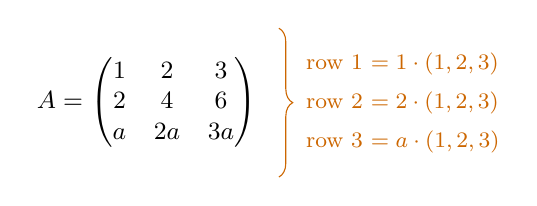
\begin{tikzpicture}[scale=0.9, every node/.style={font=\small}]
\node[anchor=west] (M) at (0,0) {$A = \begin{pmatrix} 1 & 2 & 3 \\ 2 & 4 & 6 \\ a & 2a & 3a \end{pmatrix}$};
\draw[decorate, decoration={brace, amplitude=5pt}, orange!80!black] ([xshift=5pt, yshift=1.05cm]M.east) -- ([xshift=5pt, yshift=-1.05cm]M.east);
\node[orange!80!black, right] at ([xshift=12pt, yshift=0.55cm]M.east) {\footnotesize row 1 $= 1\cdot(1,2,3)$};
\node[orange!80!black, right] at ([xshift=12pt, yshift=0.0cm]M.east) {\footnotesize row 2 $= 2\cdot(1,2,3)$};
\node[orange!80!black, right] at ([xshift=12pt, yshift=-0.55cm]M.east) {\footnotesize row 3 $= a\cdot(1,2,3)$};
\end{tikzpicture}
\end{center}

\textcolor{gray}{\small\textit{Every row is a multiple of $(1,2,3)$: the $1$-, $2$- resp.\ $a$-fold. Such a matrix has \textbf{rank $1$} (all rows ``on one line''). Just like the rank-$1$ matrix on sheet 11 (44b), almost all eigenvalues are then $0$.}}

\textbf{Step 1: Rank and eigenvalue $0$.} All rows are multiples of $(1,2,3)$ $\Rightarrow \operatorname{rank}(A) = 1$. Dimension formula: $\dim\ker(A) = 3 - 1 = 2$. So $0$ is an eigenvalue with $\text{GM}(0) = 2$.

\textbf{Step 2: the other eigenvalue.} A rank-$1$ matrix has only \emph{one} eigenvalue $\neq 0$, and it equals the trace:
\[
\operatorname{trace}(A) = 1 + 4 + 3a = 5 + 3a.
\]
The char.\ polynomial is $\chi_A(t) = t^2\,(t - (5+3a))$ -- roots $0$ (double) and $5+3a$.

\textbf{Step 3: Case distinction.}
\begin{itemize}[leftmargin=*, nosep]
    \item \textbf{$5 + 3a \neq 0$}, i.e.\ $a \neq -\tfrac{5}{3}$: eigenvalues $0$ (AM $2$, GM $2$) and $5+3a$ (AM $1$, GM $1$). GM $=$ AM everywhere $\Rightarrow$ \textbf{diagonalizable}.
    \item \textbf{$5 + 3a = 0$}, i.e.\ $a = -\tfrac{5}{3}$: now the third eigenvalue is $0$ too, i.e.\ $0$ has AM $3$. But GM$(0) = 2$ (the rank stays $1$). Since $\text{GM}(0) = 2 < 3 = \text{AM}(0)$ \textbf{not diagonalizable}.
\end{itemize}

\[
\fbox{\parbox{0.93\textwidth}{\centering
$A$ is diagonalizable \textbf{exactly when $a \neq -\tfrac{5}{3}$.} \\
For $a = -\tfrac{5}{3}$, $A$ is \emph{not} diagonalizable ($\text{GM}(0)=2 < \text{AM}(0)=3$).
}}
\]

\bigskip
\hrule
\bigskip

%% ============================================================
\subsection*{Exercise 49}
%% ============================================================

\textbf{Problem.} The sequence $(a_0, a_1, a_2, \dots)$ is given by
\[
a_0 = 4, \quad a_1 = -1, \quad a_k = 3a_{k-1} + 10 a_{k-2} \ (k \ge 2).
\]
Find an explicit formula for $a_k$ using \textbf{matrix diagonalization}.

\begin{wastun}
\begin{itemize}[leftmargin=*, nosep]
    \item Pack two consecutive terms into a vector -- then ``one step of the sequence'' becomes \emph{one} matrix multiplication $v_k = M v_{k-1}$. So $v_k = M^k v_0$. The high power $M^k$ is computed via $M = PDP^{-1}$, because $M^k = P D^k P^{-1}$ and $D^k$ is just the $k$-th power of the diagonal.
\end{itemize}
\end{wastun}

\grafik

\begin{center}
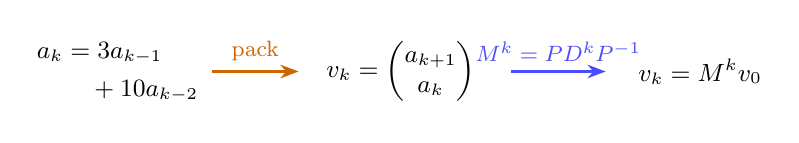
\begin{tikzpicture}[scale=1.0, >={Stealth[scale=1.0]}, every node/.style={font=\small}]
\node (rec) at (0,0) {$\begin{aligned} a_k &= 3a_{k-1} \\ &\quad + 10a_{k-2}\end{aligned}$};
\node (vec) at (3.6,0) {$v_k = \begin{pmatrix} a_{k+1} \\ a_k \end{pmatrix}$};
\node (mat) at (7.4,0) {$v_k = M^k v_0$};
\draw[->, orange!80!black, thick] (1.2,0) -- (2.3,0) node[midway, above]{\footnotesize pack};
\draw[->, blue!70, thick] (5.0,0) -- (6.2,0) node[midway, above]{\footnotesize $M^k = P D^k P^{-1}$};
\end{tikzpicture}
\end{center}

\textcolor{gray}{\small\textit{The sequence ``looks two steps back''. Packing $(a_{k+1}, a_k)$ into a vector, the matrix $M$ turns the old pair into the new one. Applying it $k$ times $=$ $M^k$ -- and that is easy via diagonalization, because $D^k$ is just the entries to the power $k$.}}

\textbf{Step 1: Vector and matrix.} Set $v_k = \begin{pmatrix} a_{k+1} \\ a_k \end{pmatrix}$. With $M = \begin{pmatrix} 3 & 10 \\ 1 & 0 \end{pmatrix}$ we have
\[
M v_{k-1} = \begin{pmatrix} 3 & 10 \\ 1 & 0 \end{pmatrix}\begin{pmatrix} a_k \\ a_{k-1} \end{pmatrix} = \begin{pmatrix} 3a_k + 10 a_{k-1} \\ a_k \end{pmatrix} = \begin{pmatrix} a_{k+1} \\ a_k \end{pmatrix} = v_k.
\]
Start vector $v_0 = \begin{pmatrix} a_1 \\ a_0 \end{pmatrix} = \begin{pmatrix} -1 \\ 4 \end{pmatrix}$, and thus $v_k = M^k v_0$.

\textbf{Step 2: Diagonalize $M$.} Char.\ polynomial:
\[
\det(M - tI) = \det\begin{pmatrix} 3-t & 10 \\ 1 & -t \end{pmatrix} = (3-t)(-t) - 10 = t^2 - 3t - 10 = (t-5)(t+2).
\]
Eigenvalues $\lambda = 5$ and $\lambda = -2$. Eigenvectors:
\begin{itemize}[leftmargin=*, nosep]
    \item $\lambda = 5$: $M - 5I = \left(\begin{smallmatrix} -2 & 10 \\ 1 & -5 \end{smallmatrix}\right)$, row $1$: $-2x + 10y = 0 \Rightarrow x = 5y$. \EV{} $(5, 1)$.
    \item $\lambda = -2$: $M + 2I = \left(\begin{smallmatrix} 5 & 10 \\ 1 & 2 \end{smallmatrix}\right)$, row $2$: $x + 2y = 0 \Rightarrow x = -2y$. \EV{} $(-2, 1)$.
\end{itemize}
\[
P = \begin{pmatrix} 5 & -2 \\ 1 & 1 \end{pmatrix},\quad D = \begin{pmatrix} 5 & 0 \\ 0 & -2 \end{pmatrix},\quad
\det P = 7,\ \ P^{-1} = \frac{1}{7}\begin{pmatrix} 1 & 2 \\ -1 & 5 \end{pmatrix}.
\]

\textbf{Step 3: $v_k = P D^k P^{-1} v_0$.} Compute right to left. First $P^{-1} v_0$:
\[
P^{-1} v_0 = \frac{1}{7}\begin{pmatrix} 1 & 2 \\ -1 & 5 \end{pmatrix}\begin{pmatrix} -1 \\ 4 \end{pmatrix} = \frac{1}{7}\begin{pmatrix} -1 + 8 \\ 1 + 20 \end{pmatrix} = \frac{1}{7}\begin{pmatrix} 7 \\ 21 \end{pmatrix} = \begin{pmatrix} 1 \\ 3 \end{pmatrix}.
\]
Then $D^k$ in front ($D^k = \left(\begin{smallmatrix} 5^k & 0 \\ 0 & (-2)^k \end{smallmatrix}\right)$):
\[
D^k P^{-1} v_0 = \begin{pmatrix} 5^k & 0 \\ 0 & (-2)^k \end{pmatrix}\begin{pmatrix} 1 \\ 3 \end{pmatrix} = \begin{pmatrix} 5^k \\ 3\,(-2)^k \end{pmatrix}.
\]
Finally $P$ in front:
\[
v_k = \begin{pmatrix} 5 & -2 \\ 1 & 1 \end{pmatrix}\begin{pmatrix} 5^k \\ 3\,(-2)^k \end{pmatrix} = \begin{pmatrix} 5\cdot 5^k - 6\,(-2)^k \\ 5^k + 3\,(-2)^k \end{pmatrix}.
\]

\textbf{Step 4: Read off $a_k$.} $a_k$ is the \emph{lower} component of $v_k$:
\[
\fbox{\parbox{0.93\textwidth}{\centering
$a_k = 5^k + 3\cdot(-2)^k.$
}}
\]

\textbf{Check:} $a_0 = 1 + 3 = 4$ \checkmark, \ $a_1 = 5 + 3\cdot(-2) = -1$ \checkmark, \ $a_2 = 25 + 3\cdot 4 = 37 = 3(-1) + 10(4)$ \checkmark.

\bigskip
\hrule
\bigskip

%% ============================================================
\subsection*{Overview: Results}
%% ============================================================

\begin{center}
\begin{tabular}{@{}ll@{}}
\toprule
Exercise & Result \\
\midrule
$47$ (a) & diagonalizable, $D = \operatorname{diag}(3,3,5)$ \\
$47$ (b) & \emph{not} diagonalizable (GM$(2)=1 <$ AM$(2)=2$) \\
$47$ (c) & diagonalizable, $D = \operatorname{diag}(0,6,6)$ \\[2pt]
$48$ (a) & diagonalizable for \textbf{all} $a \in \mathbb{R}$ \\
$48$ (b) & diagonalizable $\Leftrightarrow a \neq -\tfrac{5}{3}$ \\[2pt]
$49$ & $a_k = 5^k + 3\cdot(-2)^k$ \\
\bottomrule
\end{tabular}
\end{center}

\end{document}
